\documentclass{article}[18pt]
\usepackage[utf8]{inputenc}
\usepackage[margin=0.7in]{geometry}
\usepackage{parselines} 
\usepackage{amsmath}
\usepackage{titlesec}
\usepackage{pgfplots}
\usepackage{graphicx}
\usepackage[english]{babel}
\usepackage{fancyhdr}
\usepackage{tikz}
\usepackage{relsize}
\usetikzlibrary{scopes,quotes,arrows.meta,arrows,shapes.geometric}
\pgfplotsset{width=10cm,compat=1.9}
\usepackage{gensymb}
\usepackage{tabularx}
\titlespacing\section{0pt}{14pt plus 4pt minus 2pt}{0pt plus 2pt minus 2pt}
\newlength\tindent
\setlength{\tindent}{\parindent}
\setlength{\parindent}{0pt}
\renewcommand{\indent}{\hspace*{\tindent}}
\tikzstyle{arrow} = [thick,->,>=stealth]
\pagestyle{fancy}
\fancyhf{}
\rhead{Sam Robbins 13SE}
\lhead{A Level Physics - Further Mechanics and Thermal Physics}
\rfoot{Page \thepage}
\pgfdeclarelayer{background layer}
\pgfdeclarelayer{foreground layer}
\pgfsetlayers{background layer,main,foreground layer}

\begin{document}
\begin{center}
\underline{\huge Thermal Physics}
\end{center}
\section{Differences between heat and temperature}
\begin{tabular}{|c|c|c|}
\hline
&Heat&Temperature\\
\hline
Definition&Thermal energy(transferred from hot to cooler places)&A comparative measure of how hot something is\\
\hline
Unit&Joule&Kelvin\\
\hline
Measured using&Joulemeter&Thermometer\\
\hline
\end{tabular}
\section{Graph of heating water}
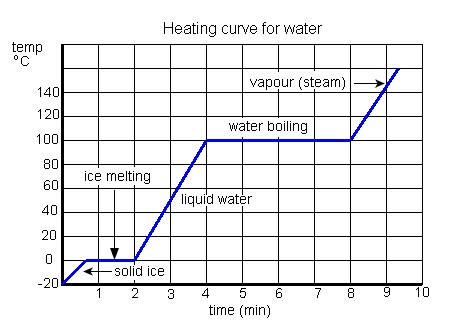
\includegraphics[width=3in]{water_heat_curve.jpg}
\section{Specific heat capacity}
\textbf{Specific heat capacity} - The energy needed to raise the temperature of 1kg of a material by 1K\\
\\
$c=\dfrac{Q}{m\Delta\theta}$\\
\\
c=Specific heat capacity - $Jkg^{-1} \ \degree C$\\
m=Mass - $kg$\\
$\Delta\theta$ = Temperature change - $\degree C$\\
Q = Heat energy - $J$
\subsection{Latent heat}
\textbf{Specific latent heat of fusion, $\mathbf{L_f}$} \quad \textcolor{red}{$Q=mL_f$}\\
The energy needed to change 1kg of a solid to a liquid without a temperature change\\
\\
\textbf{Specific latent heat of vaporisation, $\mathbf{L_v}$} \quad \textcolor{red}{$Q=mL_v$}\\
The energy needed to change 1kg of a liquid to a vapour without a temperature change
\subsection{How to determine the specific heat capacity of a metal}
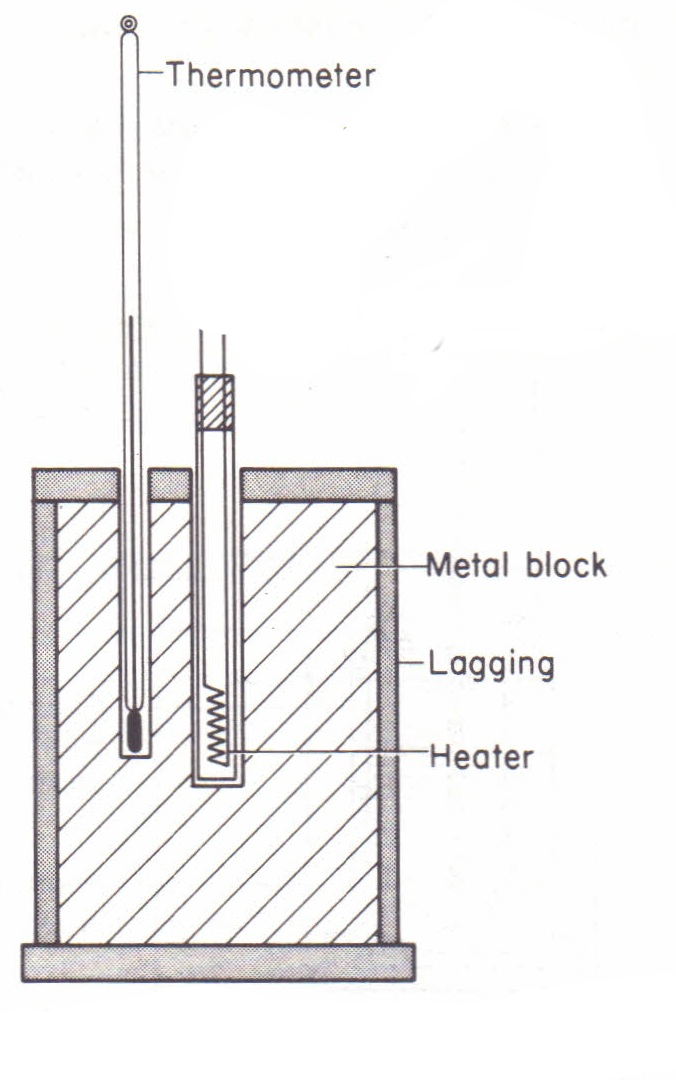
\includegraphics[width=2in]{SHC_Experiment.jpg}
\begin{enumerate}
\item Set up the experiment with a voltmeter and ammeter to determine the electrical power of the heater
\item Allow time for the heat to conduct through the metal (until there is a temperature rise)
\item Start a stopclock, record the V, I and temperature
\item Record V, I and T every 2 minutes for 20 minutes
\end{enumerate}
\section{Gas laws}
\subsection{Boyle's law}
Boyle's law - Pressure is inversely proportional to volume\\
Gases - Free moving particles, no forces\\
$$\text{Boyle's law: } P=kV^{g}$$
$$\ln(P)=\ln(k)+g\ln(V)$$
$$\text{This is in the form y=c+mx}$$
\subsection{Summary of gas laws}
\begin{tabularx}{\textwidth}{|X|X|X|X|}
\hline
Law&Proportionality&Constant&Equation\\
\hline
Boyle's&$p\propto\dfrac{1}{v}$&Temperature, moles&$p_1v_1=p_2v_2$\\
\hline
Charles'&$V\propto T$&Pressure, moles&$\dfrac{v_1}{T_1}=\dfrac{v_2}{T_2}$\\
\hline
Gay-Lussac&$p\propto T$&Volume, moles&$\dfrac{p_1}{T_1}=\dfrac{P_2}{T_2}$\\
\hline
\end{tabularx}
\newpage
\subsection{Ideal Gas equation}
$$pV=nRT$$\\
\\
p=Pressure(Pascals)\\
V=Volume($m^3$)\\
n=Number of moles\\
R=Universal gas constant=$8.31JK^{-1}\text{mol}^{-1}$\\
T=Temperature(K)
\section{Brownian Motion}
The random and unpredictable motion of a particle such as a smoke particle caused by molecules of the surrounding substance colliding at random with the particle. Its discovery provided evidence for the existence of atoms.
\section{Kinetic theory of gases}
This is a model of gas behaviour based on known laws of physics.\\
\\
On the other hand the gas laws are empirical and are based on experimental results only.\\
\subsection{Assumptions for an ideal gas}
\begin{enumerate}
\item Newton's laws of motion can be applied
\item The molecules of a particular gas are identical
\item The size of the particles are negligible compared to the distance between them
\item The molecules exert NO forces on each other, including during collision. Gravitational force is neglected. When not colliding, the particles move with constant velocity, and that velocity is random.
\item All collisions are perfectly elastic
\item The duration of the collision is negligible compared to the time between collisions.
\item There are a large number of particles so that statistics can be meaningfully applied.
\end{enumerate}
\newpage
\section{Derivation of the relationship between gas pressure and speed}

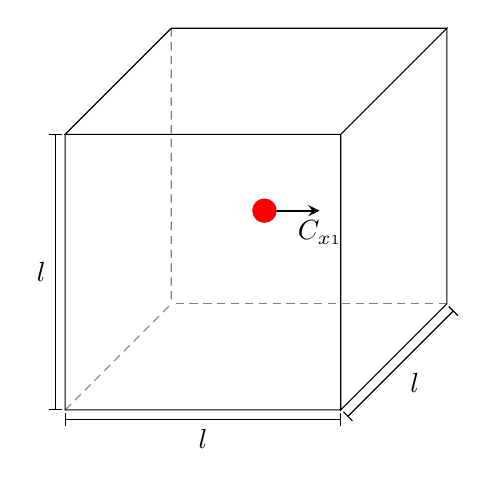
\begin{tikzpicture}[every edge quotes/.append style={auto, text=black},scale=0.7]
  \pgfmathsetmacro{\cubex}{5}
  \pgfmathsetmacro{\cubey}{5}
  \pgfmathsetmacro{\cubez}{5}
  \draw [arrow] (-1,-1,1) -- (0,-1,1) node[below] {$C_{x\mathsmaller{1}}$};
  \filldraw [red] (-1,-1,1) circle (6pt);
  \draw [draw=black, every edge/.append style={draw=black, densely dashed, opacity=.5}]
    (0,0,0) coordinate (o) -- ++(-\cubex,0,0) coordinate (a) -- ++(0,-\cubey,0) coordinate (b) edge coordinate [pos=1] (g) ++(0,0,-\cubez)  -- ++(\cubex,0,0) coordinate (c) -- cycle
    (o) -- ++(0,0,-\cubez) coordinate (d) -- ++(0,-\cubey,0) coordinate (e) edge (g) -- (c) -- cycle
    (o) -- (a) -- ++(0,0,-\cubez) coordinate (f) edge (g) -- (d) -- cycle;
  \path [every edge/.append style={draw=black, |-|}]
    (b) +(0,-5pt) coordinate (b1) edge ["$l$"'] (b1 -| c)
    (b) +(-5pt,0) coordinate (b2) edge ["$l$"] (b2 |- a)
    (c) +(3.5pt,-3.5pt) coordinate (c2) edge ["$l$"'] ([xshift=3.5pt,yshift=-3.5pt]e)
    ;
\end{tikzpicture}
\\
\textcolor{red}{Newton's $3^{\text{rd}}$ law - Every action has an equal and opposite reaction}\\
$\Delta mc=mc_{x1}--mc_{x1}=2mc_{x1}$\\
\\
\\
\textcolor{red}{Use $\text{Velocity}=\dfrac{\text{Distance}}{\text{Time}}$}\\
Time=$\dfrac{\text{Distance}}{\text{Velocity}}=\dfrac{2l}{c_{x1}}$\\
\\
\\
\textcolor{red}{Use force$=\dfrac{\text{Change in momentum}}{\text{time}}$}\\
$\text{Force}=\dfrac{\Delta mc}{\Delta t}=\dfrac{2mc{x1}}{2l/c_{x1}}=\dfrac{mc_{x1}^2}{l}$\\
\\
\\
\textcolor{red}{Use Pressure$=\dfrac{\text{Force}}{\text{Area}}$}\\
\\
$p_1=\dfrac{mc_{x1}^2/l}{l^2}=\dfrac{mc_{x1}^2}{l^3}$\\
\\
\\
\textcolor{red}{Expand for N particles}\\
$p=\Sigma p_n=p_1+p_2+p_3...+p_N$\\
\\
$p=\dfrac{mc_{x1}^2}{l^3}+\dfrac{mc_{x2}^2}{l^3}+\dfrac{mc_{x3}^2}{l^3}+\dfrac{mc_{xN}^2}{l^3}$\\
\\
$p=\dfrac{m}{l^3}(c_{x1}^2+c_{x2}^2+c_{x3}^2...+c_{xN}^2)$\\
\\
\\
\textcolor{red}{The mean of all the squares of the velocities is written as $\mathlarger{\bar{c_x^2}}$}\\
\\
$\mathlarger{\bar{c_x^2}}=\dfrac{c_{x1}^2+c_{x2}^2+c_{x3}^2...+c_{xN}^2}{N}$\\
\\
$N\mathlarger{\bar{c_x^2}}=c_{x1}^2+c_{x2}^2+c_{x3}^2...+c_{xN}^2$\\
\\
\\
\textcolor{red}{Simplify expression for pressure}\\
\\
$p=\dfrac{Nm\mathlarger{\bar{c_x^2}}}{l^3}$\\
\\
\\
\\
\textcolor{red}{Consider in 3 dimensions}\\
\\
$\mathlarger{\bar{c^2}=\bar{c_x^2}+\bar{c_y^2}+\bar{c_z^2}}$\\
\\
\\
\textcolor{red}{Average of mean square velocity for each dimension are equal}\\
\\
$\mathlarger{\bar{c_x^2}=\bar{c_y^2}=\bar{c_z^2}}$\\
\\
\\
\textcolor{red}{Simplify 3D formula}\\
\\
$\mathlarger{\dfrac{\bar{c^2}}{3}=\bar{c_x^2}=\bar{c_y^2}=\bar{c_z^2}}$\\
\\
\\
\textcolor{red}{Simplify pressure formula}\\
\\
$p=\dfrac{1}{3}\times\dfrac{Nm\mathlarger{\bar{c^2}}}{l^3}$\\
\\
\\
\textcolor{red}{Insert Density formula}\\
\\
$\rho=\dfrac{\text{Mass}}{\text{Volume}}=\dfrac{Nm}{l^3}$
\\
\\
\\
\textcolor{red}{Substitute into Pressure formula}\\
\\
$$p=\frac{1}{3}\rho\mathlarger{\bar{c^2}}$$
\newpage
\section{The relationship between kinetic energy and temperature}
$ $\\
$p=\frac{1}{3}\rho\bar{c^2}$\\
\\
\textcolor{red}{Replace density with mass divided by volume}\\
\\
$p=\frac{1}{3}\times\frac{M}{V}\bar{c^2}$\\
\\
\textcolor{red}{Multiply both sides by V and rearrange to have kinetic energy in brackets}\\
\\
$pV=\frac{2}{3}(\frac{1}{2}M\bar{c^2})$\\
\\
\textcolor{red}{Replace M(Mass of all particles) with Nm(Number of particles $\times$ the mass of one particle)}\\
\\
$pV=\frac{2N}{3}(\frac{1}{2}m\bar{c^2})$\\
\\
\textcolor{red}{Replace pV with nRT from Gas law equation}\\
\\
$nRT=\frac{2N}{3}(\frac{1}{2}m\bar{c^2})$\\
\\
\textcolor{red}{Divide both sides by n and simplify $\frac{N}{n}$ to Avagadro's constant}\\
\\
$RT=\frac{2}{3}N_A(\frac{1}{2}m\bar{c^2})$\\
\\
\textcolor{red}{Divide both sides by Avagadro's constant and simplify $\frac{R}{N_A}$ to Boltzman's Constant}\\
\\
$kT=\frac{2}{3}(\frac{1}{2}m\bar{c^2})$\\
\\
\textcolor{red}{Rearrange to have only kinetic energy on one side}\\
\\
$\frac{3}{2}kT=\frac{1}{2}m\bar{c^2}$\\
\\
\\
This shows that Average KE $\propto$ Temperature\\
\\
\section{Root mean square velocity}
$C_\text{RMS}=\mathlarger{\sqrt{\bar{c^2}}}$

\end{document}